\chapter{Nástroje pre sieťovú virtualizáciu}
\label{chap:nastroje_pre_siet_virt}

V tejto kapitole uvádzam prehľad momentálne dostupných nástrojov virtuálnych sieťových laboratórií a ich porovnaniu na základe kritérií v časti \ref{chap:porovnavacie_kriteria} - \nameref{chap:porovnavacie_kriteria}.





\section{Porovnávacie kritériá}
\label{chap:porovnavacie_kriteria}

Pri porovnávaní jednotlivých virtuálnych sieťových laboratórii boli zohľadnené tieto kritériá:
\begin{itemize}[noitemsep]
    \item Použité vývojové technológie.
    \item Podpora zariadení.
    \item Typ používateľského rozhrania.
    \item Prideľovanie portových čísel zariadeniam.
    \item Vzdialený prístup ku zariadeniam.
    \item Vytvorenie/úprava/uloženie/odstránenie topológie.
    \item Počet topológii, ktoré môže mať jeden používateľ spustených.
    \item Možnosť práce viac ľudí naraz na rovnakom projekte.
    \item Možnosť prepojiť topológiu so živou sieťou.
    \item Vývoj nástroja v budúcnosti.
    \item Vybrané výhody a nevýhody nástroja.
\end{itemize}

V nasledujúcich častiach sú popísané jednotlivé riešenia virtuálneho sieťového laboratória.





\section{Cisco Packet Tracer}

Cisco Packet Tracer je nástroj na vizualizáciu sietí vyvíjaný spoločnosťou Cisco. Je vhodný na uvedenie do problematiky sieťových technológii. Slúži na emuláciu jednoduchých aktívnych aj pasívnych sieťových prvkov a jednoduchých koncových zariadení \cite{packet_tracer}. Čo sa týka smerovačov a prepínačov, tieto sú podporované, ale iba od výrobcu Cisco a s obmedzenou funkcionalitou.

Nevýhodou je, že najnovšia verzia je prístupná výlučne pre členov \emph{Cisco Networking Academy}. K nevýhodám Cisco Packet Tracer tiež patrí, že nemá otvorený zdrojový kód čo znamená, že ho nie je možné ho ďalej rozširovať ani funkcionálne, ani pridávať podporu pre ďalšie zariadenia napr. pre sieťové zariadenia iných výrobcov alebo koncové stanice Linux/Windows. 

Na druhej strane je vyvíjaný pre platformy Windows a Linux, po emulácii aj na macOS \cite{packet_tracer_mac} a dokonca sú podporované aj mobilné platformy prostredníctvom aplikácie \emph{Packet Tracer Mobile}.

Nástroj Packet Tracer je možné používať výlučne lokálne, pretože pre tento nástroj neexistuje serverové riešenie. Vzdialený prístup, vytváranie a  topológii sa realizuje prostredníctvom grafického rozhrania aplikácie. Nástroj nevie rozlišovať rôzne typy používateľov. Je nenáročný na systémové zdroje. Umožňuje pracovať súčasne iba s jednou topológiou, pričom topológiu nie je možné prepojiť so živou sieťou.

Na obrázku \ref{obr:packet_tracer} je znázornený nástroj Cisco Packet Tracer.

\begin{figure}
    \centering
    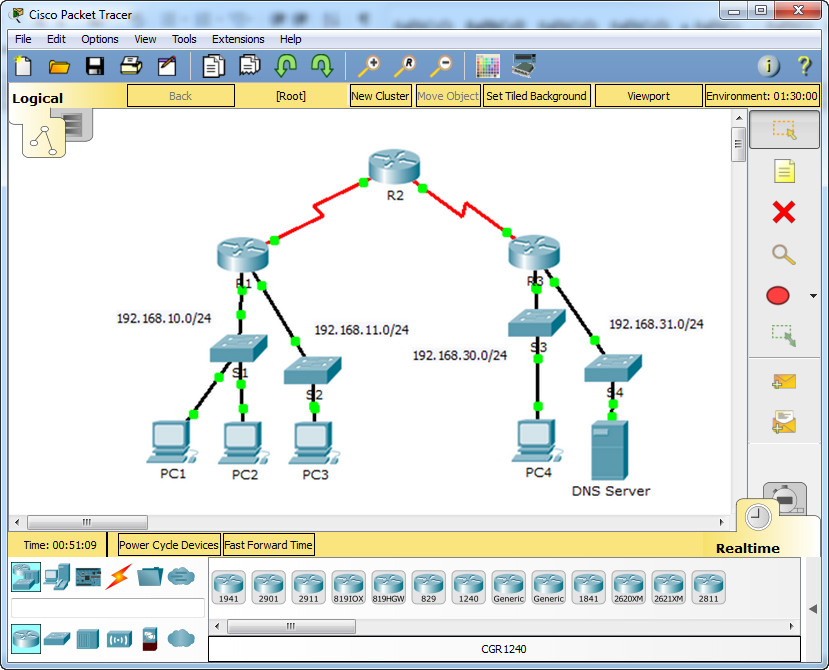
\includegraphics[width=0.65\textwidth]{packet_tracer}
    \caption{Nástroj Cisco Packet Tracer spustený v prostredí Windows}
    \cite{obr_packet_tracer}
    \label{obr:packet_tracer}
\end{figure}





\section{Dynamips/Dynagen}

Dynamips je emulátor Cisco smerovačov na Linux/Windows \cite{dynamips}. Nástroj v prevažnej mierie napísaný v jazyku C a má otvorený zdrojový kód \cite{dynamips_github}. Podporuje výlučne vybrané Cisco smerovače \cite{dynamips}. Ovláda sa cez príkazový riadok. Portové čísla na vzdialený prístup sa zariadeniam prideľujú manuálne. Vzdialený prístup k zariadeniam v topológii je realizovaný protokolom \emph{telnet}. Na vytváranie topológii sa používa jednoduchý značkovací jazyk \emph{NETMAP}.

Nástroj Dynagen tvorí nadstavbu pre platformu Dynamips a slúži na jednoduchšiu prácu s topológiami \cite{dynamips}. Topológie môže spravovať výlučne administrátor, pretože ani Dynamips, ani Dynagen nevedia rozlišovať rôzne typy používateľov. Počet topológii, ktoré môžu byť súčasne spustené je obmedzené iba výkonom servera. Na jednej topológii môžu pracovať aj viacerí študenti, tým že sa rozdelia portové čísla zariadení v topológii medzi študentov. Nástroj Dynamips umožňuje prepojiť topológiu so živou sieťou \cite{dynamips, dynamips_nil}.

V súčasnosti sa o nástroj Dynamips starajú vývojári nástroja GNS3 \cite{dynamips_github}. Na obrázku \ref{obr:dynamips_dynagen} je znázornený nástroj Dynagen.

\begin{figure}
    \centering
    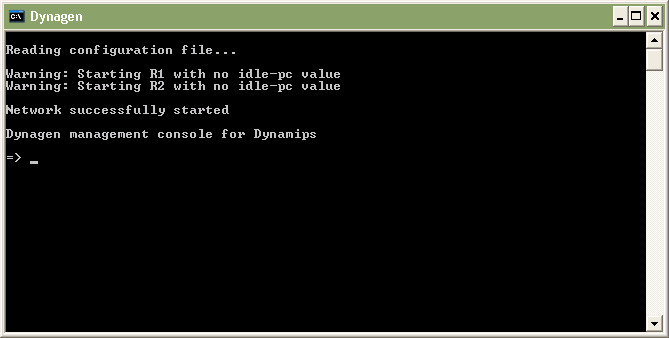
\includegraphics[width=0.75\textwidth]{dynamips_dynagen}
    \caption{Nástroj Dynagen spustený v prostredí Windows} \cite{obr_dynamips_dynagen}
    \label{obr:dynamips_dynagen}
\end{figure}





\section{WEB-IOU}

WEB-IOU, je simulačný nástroj pre platformu Linux, ktorý podporuje iba Cisco zariadenia na platforme IOU - IOS on Unix \cite{webiou_firewall_cx}. Jeho hlavnou výhodou je podpora Cisco prepínačov, ktorá v nástroji Dynamips/Dynagen chýba. Jeho autorom je Andrea Dainese \cite{webiou_github, webiou_unetlab_unetlabv2}. Nástroj je v prevažnej mierie napísaný v jazykoch PHP a JavaScript \cite{webiou_github}. Je vhodný na trénovanie pri certifikáciách CCNP a do istej miery aj CCIE.

Spravuje sa cez príkazový riadok. Používateľovi je dostupné web rozhranie. Portové čísla na vzdialený prístup sa zariadeniam prideľujú automaticky. Vzdialený prístup k zariadeniam v topológii je realizovaný protokolom \emph{telnet}. Na vytváranie topológii sa používa jednoduchý značkovací jazyk \emph{NETMAP}. Topológie môže spravovať ktokoľvek, kto má prístup k web rozhraniu, pretože ani tento nástroj nevie rozlišovať rôzne typy používateľov. Počet topológii, ktoré môžu byť súčasne spustené je obmedzené iba výkonom servera. Napriek tomu môžu na jednej topológii môžu pracovať aj viacerí študenti rovnakým spôsobom, ako pri nástroji Dynamips/Dynalab. Nástroj WEB-IOU umožňuje prepojiť topológiu so živou sieťou \cite{webiou_real_network}. 

V súčasnosti sa už nástroj nevyvíja. Na obrázku \ref{obr:webiou} je znázornené webové rozhranie nástroja WEB-IOU.

\begin{figure}
    \centering
    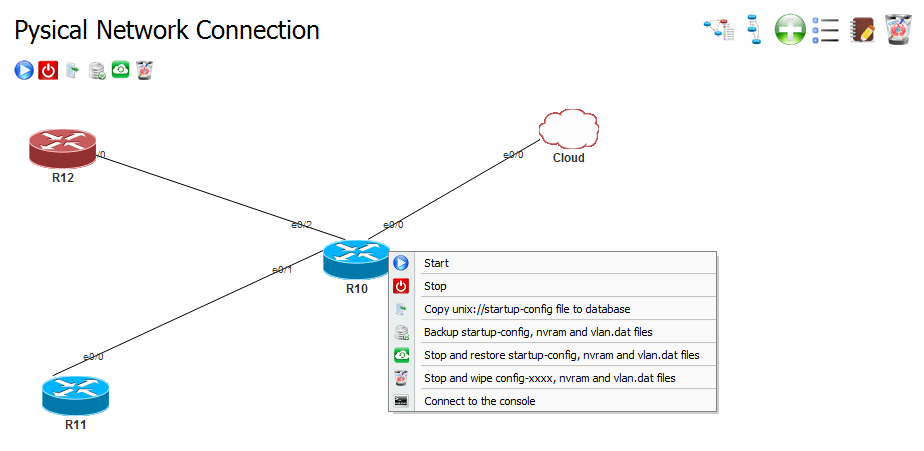
\includegraphics[width=0.75\textwidth]{webiou}
    \caption{Webové rozhranie nástroja WEB-IOU} \cite{obr_webiou}
    \label{obr:webiou}
\end{figure}





\section{Cisco VIRL}

Cisco VIRL, Virtual Internet Routing Lab, je komerčný simulačný nástroj sietí vyvíjaný spoločnosťou Cisco. Podporuje nielen Cisco smerovače a prepínače, ale aj zariadenia iných výrobcov. Nástroj je postavený na platforme Linux (Debian) a je dostupný ako virtuálny stroj pre rôzne platformy. Je vhodný na trénovanie pri certifikáciách CCNP a do istej miery aj CCIE \cite{virl_cisco}.

Výhodou oproti iným nástrojom je možnosť pridať vybrané podporované zariadenia, napr. koncové zariadenia, do topológie ako LXC kontajner \cite{virl_cisco}.

Nevýhodou je, že nepodporuje Dynamips/Dynagen emuláciu, takže na ňom nie je možné využiť existujúce virtuálne zariadenia na katedre \cite{virl_cisco}. Spomínaná integrácia zariadení iných výrobcov je síce možná, ale nemusí byť jednoduchá.

Spravuje sa cez príkazový riadok. Používateľovi je dostupné web rozhranie. Portové čísla na vzdialený prístup sa zariadeniam prideľujú automaticky \cite{virl_interfacett_1}. Vzdialený prístup k zariadeniam v topológii je realizovaný protokolmi \emph{telnet} a \emph{ssh}, po úprave aj \emph{vnc} \cite{virl_ciscoskills, virl_speaknetworks}. Na vytváranie topológii sa používa Nástroj \emph{VM Maestro}. Ten poskytuje možnosť, vopred si nakonfigurovať zariadenie podľa zvolených scenárov pomocou funkcie \emph{AutoNetkit}. Aj napriek tomu, že VIRL poskytuje pomerne široké možnosti na konfiguráciu Cisco zariadení a topológii, jeho používanie je pomerne obtiažne, hlavne pri vytváraní topológii \cite{virl_interfacett_1, virl_interfacett_2}. Cisco VIRL rozlišuje používateľov podľa typu na administrátorov a používateľov \cite{virl_cisco_features}. Počet topológii, ktoré môžu byť súčasne spustené je obmedzené iba výkonom servera. Napriek tomu môžu na jednej topológii môžu pracovať aj viacerí študenti rovnakým spôsobom, ako pri nástroji Dynamips/Dynalab \cite{virl_interfacett_2}. Nástroj tiež umožňuje prepojiť topológiu so živou sieťou \cite{virl_speaknetworks}. 

Nástroj v súčasnosti existuje iba vo verzii \emph{Personal Edition} s licenciou na 20 zariadení, čo výrazným spôsobom obmedzuje jeho využitie vo vyučovaní. V minulosti existovali aj verzie \emph{Personal Edition} s licenciou na 30 zariadení a \emph{Academic Edition}. Rozdiel medzi Personal a Academic Edition bol iba ten, že Academic Edition bol prístupný učiteľom a študentom za výhodnejšiu cenu. Podporované funkcionality boli zhodné v oboch verziách \cite{virl_edition_differences}. Na obrázkoch \ref{obr:virl_vmmaestro} a \ref{obr:virl_web} je znázornený nástroj VM Maestro a webové rozhranie Cisco VIRL.

\begin{figure}
    \centering
    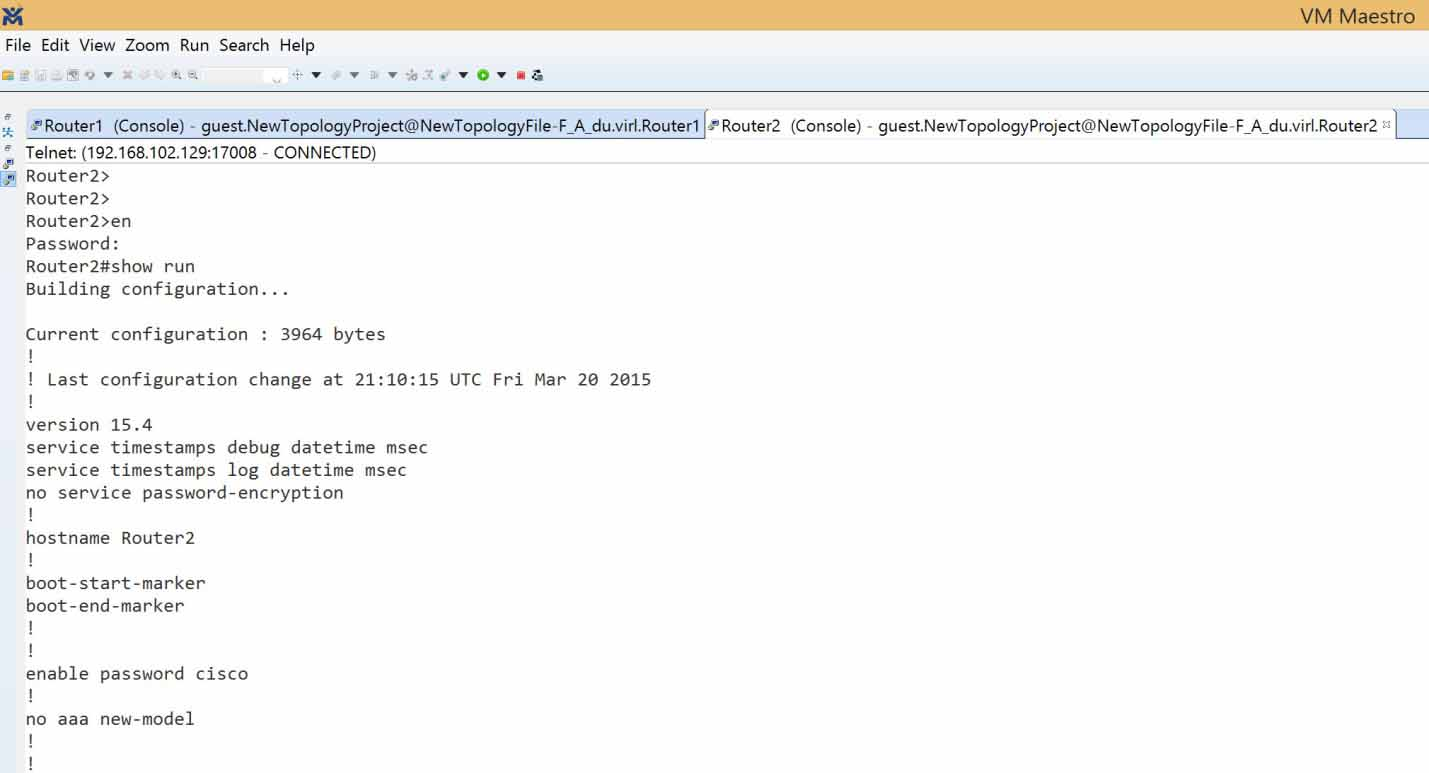
\includegraphics[width=0.75\textwidth,trim={0 0 5cm 0},clip]{virl_vmmaestro}
    \caption{VM Maestro} \cite{obr_virl_vmmaestro}
    \label{obr:virl_vmmaestro}

    \vspace{4cm}

    \centering
    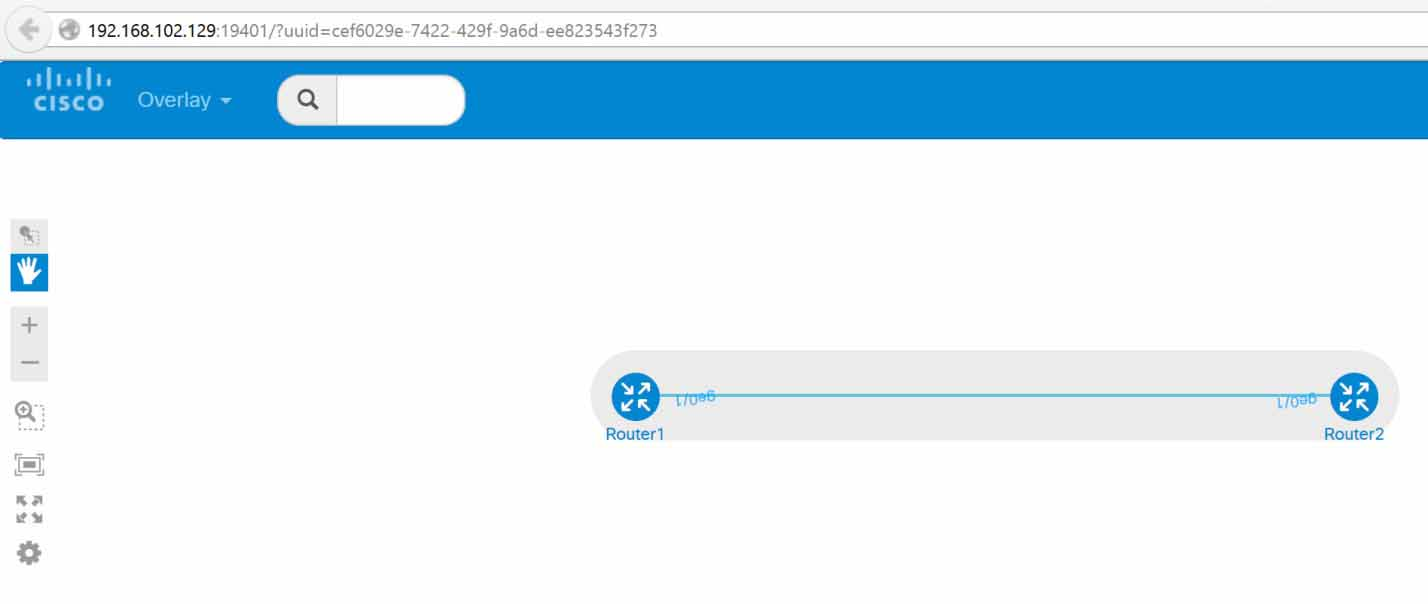
\includegraphics[width=0.75\textwidth]{virl_web}
    \caption{Cisco VIRL web rozhranie} \cite{obr_virl_web}
    \label{obr:virl_web}
\end{figure}





\section{ViRo2}

ViRo2 je virtuálne laboratórium vytvorený na Katedre informačných sietí na Fakulte riadenia a informatiky Žilinskej univerzity v Žiline. Nástroj vznikol ako výsledok diplomovej práce Ing. Petra Hadača, pričom pokračoval v predchádzajúcej verzii nástroja, ViRo. Nástroj je postavený na platforme Linux. Využíva technológie tzv. \emph{LAMP Stack} servera: Linux, Apache, MySQL, PHP (Drupal). Využíva virtualizáciu pomocou QEMU/KVM a Dynamips. Jeho hlavnou výhodou je možnosť rezervovať si topológiu. Ďalšou možnou nevýhodou je, že webové rozhranie stavia na platforme Drupal, ktorého popularita výrazne klesá \cite{stackoverflow_survey}. Okrem toho, takéto nástroje pre správu webovej stránky, ako napr. Wordpress, Joomla a.i. sa môžu stať potenciálnym bezpečnostným rizikom. \cite{incapsula_cms}

Spravuje sa prostredníctvom web rozhrania, SSH alebo VNC prístupu. Používateľom je dostupné webové rozhranie. Portové čísla na vzdialený prístup sa zariadeniam dajú nastaviť manuálne. Vzdialený prístup k zariadeniam v topológii je realizovaný viacerými spôsobmi: pomocou nástroja \emph{virsh}, aplikáciou \emph{Virtual Machine Manager} prístupnou cez \emph{vnc}, \emph{noVNC} serverom alebo SSH tunelom. Vytváranie topológii a správu zariadení sa používa grafický nástroj \emph{Virtual Machine Manager}. Nástroj ViRo2 vie rozlišovať používateľov s rolou \emph{administrátor}, \emph{učiteľ} a \emph{študent}. Topológie môže vytvárať iba používateľ s rolou \emph{učiteľ} alebo \emph{administrátor}. Počet topológii, ktoré môžu byť súčasne spustené je obmedzené iba výkonom servera. Napriek tomu môžu na jednej topológii môžu pracovať aj viacerí študenti rovnakým spôsobom, ako pri nástroji Dynamips/Dynalab. Nástroj umožňuje prepojiť topológiu so živou sieťou pomocou \emph{bridge} rozhrania \cite{viro_hadac}.





\section{UNetLab}

UNetLab, Unified Networking Lab, skrátene UNL, je open-source  simulačný nástroj pre platformu Linux, ktorý integruje všetky vyššie uvedené technológie najednom mieste: Dynamips, Cisco IOU aj zariadenia tretích strán použitím QEMU/KVM technológie. Nástroj je postavený na platforme Linux. Jeho autorom je Andrea Dainese. V prevažnej mierie je napísaný v jazykoch PHP a JavaScript \cite{webiou_unetlab_unetlabv2, unetlab_github}. Je vhodný nielen na trénovanie pri Cisco certifikáciách, ale aj na testovanie vzájomnej spolupráce zariadení od rôznych výrobcov.

Spravuje sa cez príkazový riadok. Používateľovi je dostupné web rozhranie. Portové čísla na vzdialený prístup sa zariadeniam prideľujú automaticky. Vzdialený prístup k zariadeniam v topológii je realizovaný protokolom \emph{telnet} alebo \emph{vnc}. Topológie sa vytvárajú vo webovom rozhraní prepájaním uzlov medzi sebou pomocou myši, pričom sa na pozadí sa generuje súbor v značkovacom jazyku \emph{NETMAP}, ktorý o.i. definuje zariadenia v topológii. Topológie môže ktokoľvek, kto má prístup k web rozhraniu, pretože ani tento nástroj nevie rozlišovať rôzne typy používateľov, hoci v istej verzii nástroja táto funkcia bola podporovaná \cite{unetlab_github}. Počet topológii, ktoré môžu byť súčasne spustené je obmedzené iba výkonom servera. Napriek tomu môžu na jednej topológii môžu pracovať aj viacerí študenti rovnakým spôsobom, ako pri nástroji Dynamips/Dynalab. Jeden používateľ môže mať otvorenú práve jednu topológiu, ktorá sa dá zatvoriť až vtedy, keď v nej nie sú spustené žiadne zariadenia. Nástroj UNetLab tiež umožňuje prepojiť topológiu so živou sieťou pomocou \emph{bridge} rozhrania \cite{webiou_real_network}.

Vývoj tohto nástroja bol zastavený. UNetLab ďalej vyvíjala iná skupina vývojárov, ktorý nástroj premenovala na EVE-ng a migrovala ho z platformy Ubuntu 14.04 na Ubuntu 16.04. Jeho pôvodný autor následne začal s vývojom ďalšej verzie nástroja UNetLab, UNetLabv2, ktorému sa venujeme v časti \ref{chap:unetlabv2} - \nameref{chap:unetlabv2}. Na obrázku \ref{obr:unetlab_web} je znázornené webové rozhranie nástroja UNetLab.

\begin{figure}
    \centering
    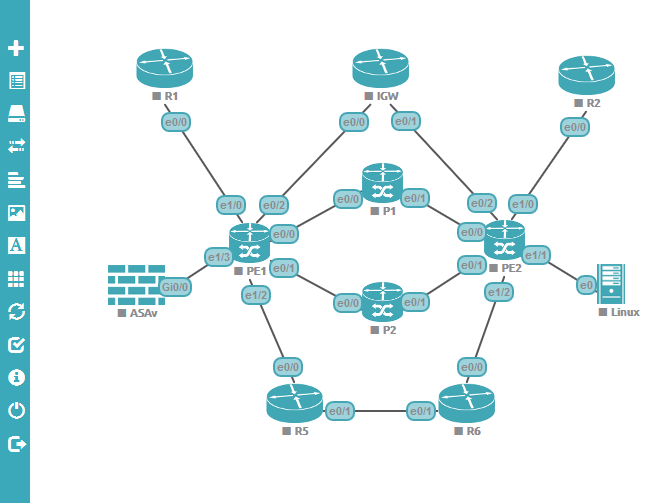
\includegraphics[width=0.75\textwidth]{unetlab_web}
    \caption{Webové rozhranie nástroja UNetLab}
    \cite{obr_unetlab_web}
    \label{obr:unetlab_web}
\end{figure}





\section{EVE-ng}
\label{chap:virt_lab_eve_ng}

EVE-ng je simulačný nástroj sietí, ktorý vznikol ako klon a nasledovník nástroja UNetLab. Celkovou funkcionalitou, až na niektoré zmeny, napr. použitie MySQL namiesto SQLite, pridaná podpora pre ďalšie zariadenia), a vzhľadom webového rozhrania sa preto veľmi podobá na svojho predchodcu. Nástroj je postavený na platforme Linux a vyvíjaný prevažne v jazykoch JavaScript a PHP. Web rozhranie je realizované ako webová aplikácia s použitím framework nástroja \emph{Angular JS} a \emph{Twitter Bootstrap} \cite{eve_ng_technologies}.

EVE-ng sa v priebehu marca 2018 rozdelilo na tri verzie: Community, Professional a Learning Centre. Community verzia je open-source, aj keď \emph{gitlab} repozitár bol neprístupný pre verejnosť v priebehu novembra/decembra 2017. Napriek tomu sú na serveri všetky súbory prístupné a upravovateľné. Túto verziu je možné slobodne šíriť a upravovať. Verzia Professional obsahuje niektoré funkcionality, ktoré uľahčujú prácu s nástrojom, ale vývojári sa rozhodli spoplatniť ju. Learning Centre verzia obsahuje funkcionality na nasadenie do produkčného prostredia, ako je napr. rozdelenie používateľov do používateľských rolí. Podrobný zoznam podporovaných funkcii v jednotlivých verziách je dostupný v \cite{eve_ng_versions_table} a \cite{eve_ng_versions_list}.

Vzhľad webového rozhrania EVE-ng je znázornený na obrázku \ref{obr:eve_ng_web}. Rozdiely jednotlivých verzii EVE-ng sú znázornené v tabuľke \ref{tab:eve_ng_versions}.

\begin{figure}
    \centering
    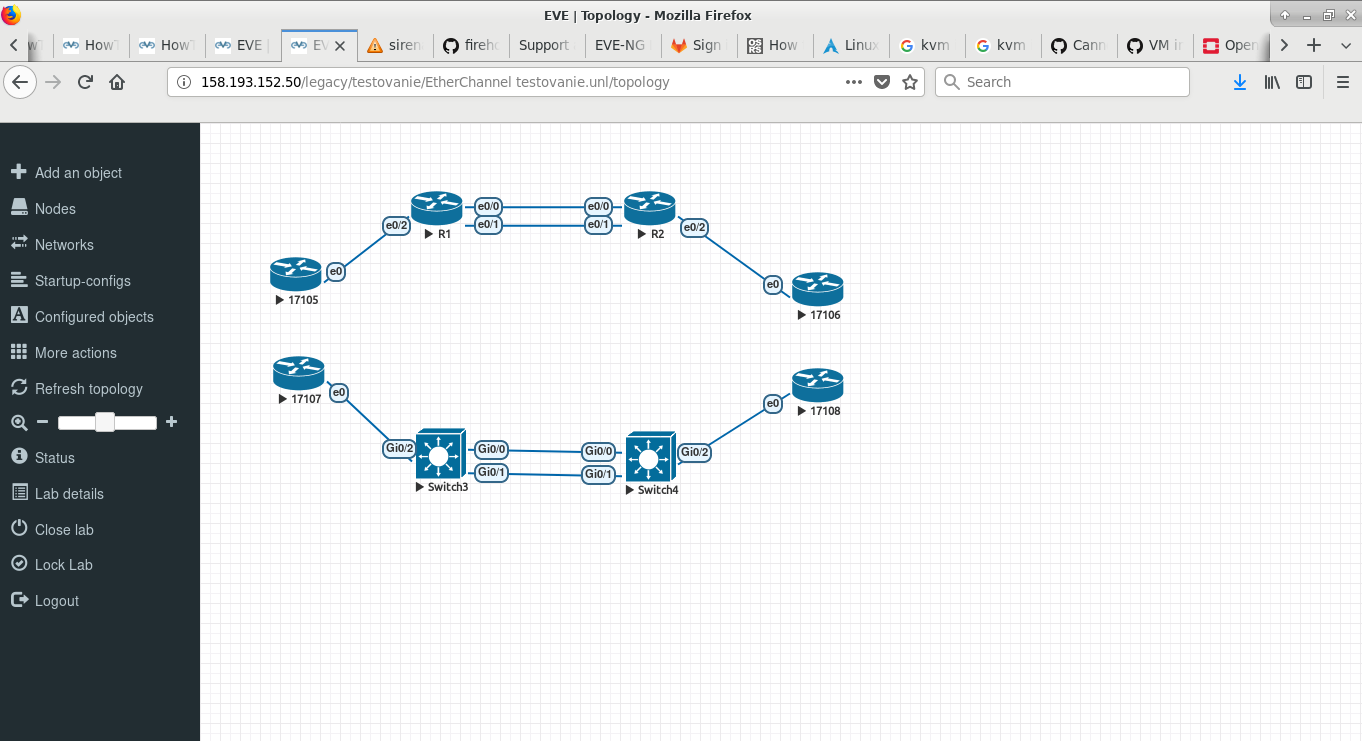
\includegraphics[width=0.75\textwidth,trim={0 2cm 17cm 5cm},clip]{eve_ng_web}
    \caption{Webové rozhranie nástroja EVE-ng}
    \label{obr:eve_ng_web}
\end{figure}

Z tabuľky vyplýva, že verzie \emph{Community} je ako jediná bezplatná. Najväčšími výhodami ostatných verzii je rozdelenie používateľov do používateľských rolí a izolácia ich súborov (iba v \emph{Learning Centre}), zatvorenie topológie s už spustenými zariadeniami, prehľad zatvorených topológii so spustenými zariadeniami a zvýšený limit na počet spustených zariadení pre topológiu.

Doplnením a rozšírením funkcionality EVE-ng Community verzie je venovaná kapitola \ref{chap:eve_ng_uprava_zdroj_kodov} - \nameref{chap:eve_ng_uprava_zdroj_kodov}.

\newpage

\begin{longtable}{| m{3cm} | m{2cm} | m{2cm} | m{2cm} | m{4cm} |}
\caption{Porovnanie EVE-ng verzii}
\cite{eve_ng_versions_table}
\label{tab:eve_ng_versions} \\
\hline
Funkcia/Verzia                                      & Community         & Professional    & Learning Center      & Popis                                                                                                   \\ \hline
Cena                                                 & zadarmo              & 99 EUR  & 99 EUR & Pre Learning Center verziu platí, že pre každého ďalšieho používateľa, ktorý by sa chcel prihlásiť pod rovnakým používateľským menom, treba zaplatiť rovnakú sumu. Táto funkcia je vhodná pri spolupráci na rovnakej topológii.
\\ \hline
Používateľské role                                          & admin        & admin      & admin, user (študent), editor (učiteľ)  & Obmedzenia pre webových používateľov EVE-ng \\ \hline
Samostatný adresár pre každého používateľa                                  & Nie                & Nie              & Áno                  & Používateľ nemôže vidieť súbory a adresáre iného používateľa, iba svoje vlastné \\ \hline
Používateľ nemôže upravovať súbory                                 & Nie                & Nie              & Áno                  & Používateľ s rolou \emph{user} nemôže upravovať súbory ani prvky v topológii                                                                             \\ \hline
Adresár so zdieľanými topológiami                                     & Nie                & Nie              & Áno                  & Adresár so zdieľanými topológiami je viditeľný pre všetkých používateľov                                                                       \\ \hline
Platnosť používateľského účtu         & Nie                & Nie              & Áno                  & Možnosť nastaviť platnosť používateľského účtu v kalendári                         \\ \hline
Časomiera                                             & Nie                & Áno             & Áno                  & Do topológie je možné pridať časomieru na sledovanie trvania na vypracovanie                                                                                          \\ \hline
Adresár so spustenými topológiami                                   & Nie                & Áno             & Áno                  & Používatelia s rolou \emph{admin} a \emph{editor} môžu zatvoriť topológiu so spustenými zariadeniami a otvoriť ďalšiu topológiu. Topológie so spustenými zariadeniami sa objavia v osobitnom adresári.       \\ \hline
Node limit per lab                                    & 63                & 1024            & 1024                 & Limit of nodes to run per lab                                                                                 \\ \hline
Rozsah TCP portov                                             & pevný - 128 pre každého používateľa & dynamický - 1-65000 & dynamický - 1-65000      & Automatická voľba TCP portu na pre vzdialené pripojenie cez telnet                                     \\ \hline
Lokálne odchytávanie nástrojom Wireshark                               & Áno               & Nie              & Nie                   & Lokálne odchytávanie použitím SSH a \emph{root} používateľského účtu                          \\ \hline
Lokálny telnet klient                                   & Áno               & Áno             & Áno                  & Lokálny telnet klient musí byť nainštalovaný na počítači.                                                           \\ \hline
Lokálny VNC klient                                      & Áno               & Áno             & Áno                  & Lokálny VNC klient musí byť nainštalovaný na počítači.                                                              \\ \hline
Integrovaný nástroj Wireshark                                  & Nie                & Áno             & Áno                  & Nástroj Wireshark je integrovaný na serveri a je možné ho pridať do topológie na odchytávanie prevádzky. Pre verziu Community je dostupné iba odchytávanie pomocou lokálne nainštalovaného nástroja Wireshark.                                                                                   \\ \hline
Podpora Docker kontajnerov                              & Nie                & Áno             & Áno                  & Spúšťanie CLI aj grafických Docker kontajnerov.                                                                                      \\ \hline
Prepájanie už spustených zariadení (hot connections) & Nie                & Áno             & Áno                  & Pridávanie a odstraňovanie liniek medzi zariadeniami v topológii pre spustené zariadenia.                           \\ \hline
NAT Cloud                                             & Nie                & Áno             & Áno                  & Integrovaná NAT sieť umožňuje pripojiť zariadenia v topológii k internetu. Zariadeniam je následne pomocou DHCP pridelená IP adresa z rozsahu 169.254.254.0/24 \\ \hline
Desktop Console vo webovom rozhraní                                  & Nie                & Áno             & Áno                  & Integrovateľný Docker kontajner na správu koncových zariadení                          \\ \hline
Viacero spúšťacích konfigurácii pre topológiu            & Nie                & Áno             & Áno                  & Možnosť vytvárať a spúšťať topológie s rôznymi spúšťacími konfiguráciami pre jednotlivé zariadenia v topológii.                     \\ \hline
Exportovanie a importovanie konfigurácii z topológie     & Nie                & Áno             & Áno                  & Exportovanie a importovanie jednej alebo viacerých konfigurácii pre zariadenia v topológii na/z lokálny počítač                                             \\ \hline  
\end{longtable}





\section{GNS3}

GNS3, Graphical Network Simulator 3, je open-source sieťový simulátor sietí. Integruje všetky virtualizačné technológie najednom mieste: Dynamips, Cisco IOU aj zariadenia tretích strán (QEMU). Od verzie 1.5 sú v GNS3 podporované aj Docker kontajnery, čo je veľkou výhodou oproti iným nástrojom, pretože Docker kontajnery potrebujú menej systémových prostriedkov \cite{gns3_docker}.

GNS3 sa skladá z klientskej a serverovej časti. Klientská časť pozostáva z aplikácie \emph{GNS3 Client} a je celá napísaná v jazyku Python \cite{gns3_gui_github}. Klientská aplikácia je multiplatformová t.j. je kompatibilná s platformami Windows, Linux a macOS. Existuje aj klientská webová aplikácia \emph{gns3-web} \cite{gns3_web_github}. Tak by sa GNS3 priblížila k EVE-ng, keďže aj v EVE-ng sa používa webové rozhranie na prácu s topológiou.

Serverová časť môže byť realizovaná ako serverová aplikácia \emph{GNS3 Server}, ako virtuálny stroj \emph{GNS3 VM} alebo ako vzdialený server.

Serverová aplikácia \emph{GNS3 Server} sa spustí predvolene pri spustení klientskej aplikácie. Rovnako, ako GNS3 klientská aplikácia, aj serverová aplikácia je napísaná celá v jazyku Python \cite{gns3_server_github}.

GNS3 VM aj vzdialený server je postavený na platforme Linux. Vzdialený server nemusí nutne byť fyzický server, na ktorom je nasadený GNS3 server. Môže byť v ľubovoľnom virtualizačnom nástroji, ale odporúčaný je VMware, pretože podporuje vnorenú virtualizáciu, čo VirtualBox doposiaľ nepodporuje \cite{nested_virtualization}.

GNS3 VM resp. vzdialený server sa spravuje cez príkazový riadok. Používateľovi je dostupná klientská aplikácia. Portové čísla na vzdialený prístup sa zariadeniam prideľujú automaticky, avšak je možné manuálne meniť rozsah, v akom sa majú portové čísla automaticky prideľovať, dokonca umožňuje aj manuálnu zmenu čísla portu pre jednotlivé zariadenia \cite{gns3_console_ports, gns3_console_ports_remote}. Vzdialený prístup k zariadeniam v topológii je realizovaný protokolom \emph{telnet}, \emph{vnc} alebo \emph{rdp}. Topológie sa vytvárajú v klientskej aplikácii prepájaním uzlov medzi sebou pomocou myši. V predvolenom nastavení sú všetky topológie na GNS3 VM / vzdialenom serveri zdieľané a môže ich meniť ktokoľvek, kto má k serveru z GNS3 klientskej aplikácie, pretože v predvolenom nastavení nástroj nevie rozlišovať rôzne typy používateľov ani ich izolovať. Počet topológii, ktoré môžu byť súčasne spustené je obmedzené iba výkonom servera. Napriek tomu môžu na jednej topológii môžu pracovať aj viacerí študenti tým, že si otvoria rovnaký projekt na vzdialenom serveri. Zmeny v takejto zdieľanej topológii sa prejavia okamžite všetkým používateľom, ktorí majú túto topológiu práve otvorenú. Jeden používateľ môže mať spustených aj viacero topológii, klientská aplikácia však dovoľuje pracovať iba s jednou naraz. Aj GNS3, podobne ako aj ďalšie nástroje, umožňuje prepojiť topológiu so živou sieťou pomocou \emph{bridge} rozhrania alebo \emph{NAT} siete.

Vývoj tohto nástroja stále pokračuje. Na obrázku \ref{obr:gns3_client} je znázornená klientská aplikácia GNS3 Client.

\begin{figure}
    \centering
    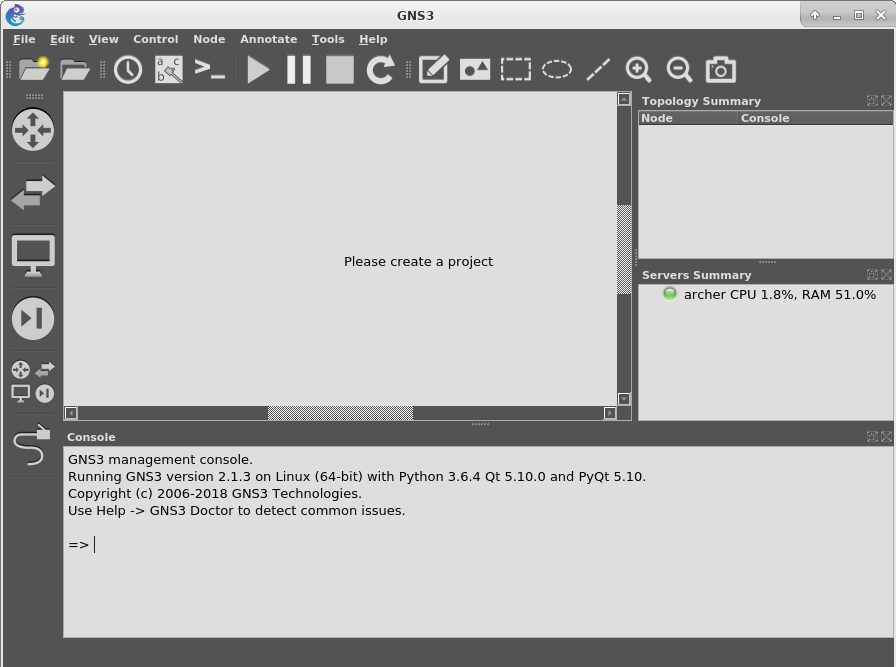
\includegraphics[width=0.75\textwidth]{gns3_client}
    \caption{Klientská aplikácia GNS3}
    \label{obr:gns3_client}
\end{figure}





\section{UNetLabv2}
\label{chap:unetlabv2}

UNetLabv2 je nasledovníkom nástroja UNetLab. Je postavený na platforme Docker kontajnerov. Jednotlivé úlohy sú distribuované naprieč kontajnermi. To zaisťuje lepšiu škálovateľnosť pri zachovaní rovnakej funkcionality. Zatiaľ ešte nie je verejne nedostupný. \cite{webiou_unetlab_unetlabv2}

Architektúra nástroja UNetLabv2 je znázornená na obrázku \ref{obr:unetlabv2_arch}

\begin{figure}
    \centering
    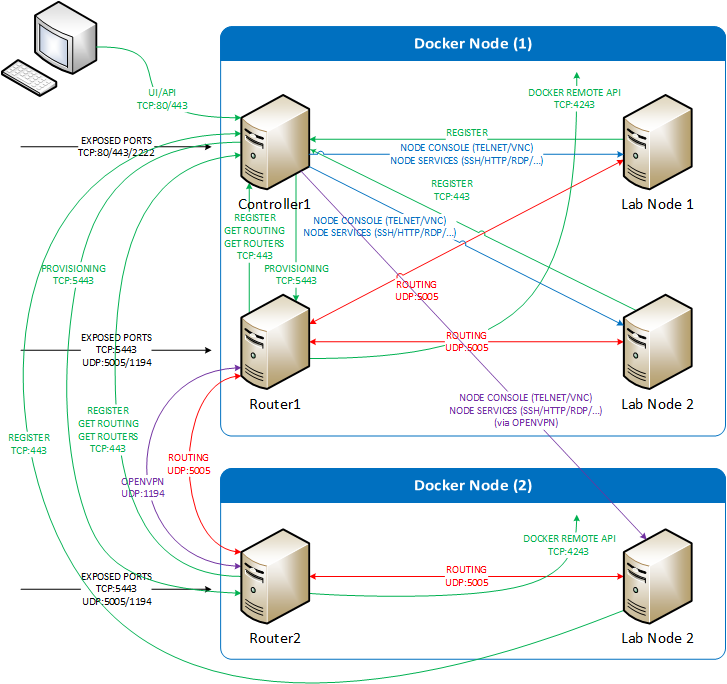
\includegraphics[width=0.8\textwidth]{unetlabv2_arch}
    \caption{Architektúra nástroja UNetLabv2} \cite{obr_unetlabv2_arch}
    \label{obr:unetlabv2_arch}
\end{figure}





\section{Vyhodnotenie}

Z vyššie uvedených nástrojov má zmysel zaoberať sa nástrojmi EVE-ng a GNS3 z nasledovných dôvodov:
\begin{itemize}[noitemsep]
    \item Open-source vývoj oboch nástrojov umožňuje ich používanie bez poplatkov, obáv o porušenie licenčných podmienok a poskytuje možnosť upravovať ich podľa vlastných požiadaviek.
    \item Podpora rôznych virtualizačných technológii.
    \item Podpora zariadení od rôznych výrobcov.
    \item Jednoduché ovládanie.
\end{itemize}

V priebehu projektu sme sa preto zamerali na nástroje GNS3 a EVE-ng. Počas neho sa však ukázalo, že GNS3 nie je vhodná pre vzdialené použitie, preto sme sa týmto nástrojom ďalej nezaoberali. V čase skúmania bol nástroj GNS3 vo verzii 1.5.3. Keď sme skúšali použiť GNS3 ako vzdialený server, klientská aplikácia sa na GNS3 vzdialený server nevedela pripojiť, hoci sme postupovali podľa návodov na GNS3 stránke a pri testovaní nestála v pripojení na server žiadna prekážka napr. firewall.

Napriek tomu je GNS3 silným nástrojom, schopný konkurovať EVE-ng. V tabuľke \ref{tab:gns3_eve_ng_porovnanie} porovnávame jednotlivé výhody a nevýhody oboch nástrojov.

% Please add the following required packages to your document preamble:
% \usepackage{multirow}
% \usepackage{longtable}
% Note: It may be necessary to compile the document several times to get a multi-page table to line up properly
\begin{longtabu} to \textwidth {| X[0.5,lm] | X[1.0,lm] | X[1.0,lm] |}
\caption{Porovnanie GNS3 a EVE-ng}
\label{tab:gns3_eve_ng_porovnanie} \\
\cline{2-3}
\multicolumn{1}{c}{} & \multicolumn{1}{|c}{\textbf{GNS3}}    & \multicolumn{1}{|c|}{\textbf{EVE-ng}}    \\ \hline
\endfirsthead
%
\endhead
%
\makecell[cc]{\multirow{8}{*}[-3cm]{\textbf{Výhody}}}   & \multicolumn{2}{c|}{Možnosť nasadenia ako vzdialené servery}                                                                                                                                                                                                                                                                                                                                                                                                                       \\ \cline{2-3} 
                                   & \multicolumn{2}{c|}{Podpora viacerých používateľov (multi-user)}                                                                                                                                                                                                                                                                                                                                                                                                                  \\ \cline{2-3} 
                                   & \multicolumn{2}{c|}{\makecell{Eventuálne možný import používateľských účtov na server z LDAP: \\ -pre GNS3 do operačného systému \\
                                   -pre EVE-ng do Linuxu alebo MySQL databázy}}                                                                                                                                                                                                                                                                                                                    \\ \cline{2-3}
                                   & \makecell[lc]{Multiplatformová klientská \\aplikacia (Windows/Linux/macOS)}                                                                                                                                                                                       & Multiplatformový klient - webová aplikácia                                                                                                                                                                                      \\ \cline{2-3} 
                                   & Natívna podpora Docker kontajnerov                                                                                                                                                                                                             & \makecell[lc]{Podpora Telnet/VNC vzdialeného\\ pripojenia ku zariadeniam cez\\ HTML5 reverse proxy server\\ (Apache Guacamole) - na\\ klientský počítač netreba\\ inštalovať  nič, okrem webového\\ prehliadača a nástroja Wireshark}                      
                                   
                                   \\ \cline{2-3} 
                                   
                                   & \makecell[lc]{Podpora viacerých používateľov\\ pri práci na spoločnom projekte\\ - pri práci viacerých používateľov\\ na jednom projekte sa topológia\\ sa pri zmene okamžite aktualizuje\\ všetkým používateľom a všetci\\ môžu pracovať so zariadeniami z\\ GNS3 klienta}
                                   
                                   & Podpora viacerých používateľov pri práci na spoločnom projekte - topológia sa aktualizuje až po kliknutí na \emph{Refresh topology}, nie okamžite po jej zmene                                                                       \\ \cline{2-3} 
                                   & \makecell[lc]{Lepšia škálovateľnosť oproti \\EVE-ng - možnosť vytvoriť\\ GNS3 cluster}                                                                                                                                                                             & Podpora viacerých používateľov - autentifikácia používateľa menom a heslom                                                                                                                                                      \\ \cline{2-3} 
                                   & \makecell[lc]{Širšie možnosti nastavenia \\z GNS3 klienta} & Užšie možnosti nastavenia z EVE-ng webového rozhrania.                                                                                                                                                                                                                                 \\ \hline
\makecell[cc]{\multirow{7}{*}[-4cm]{\textbf{Nevýhody}}} & \makecell[lc]{Nutnosť inštalácie samostatnej \\ klientskej aplikacie}                                                                                                                                                                                            & Pomalé HTML5 webové rozhranie                                                                                                                                                                                                   \\ \cline{2-3} 
                                   & Zložitejšia konfigurácia autentifikácie a izolácie používateľov                                                                                                                                                                                & \makecell[lc]{V Community verzii sú\\ používatelia sú typu \emph{administrátor}\\ a nie sú nijako od seba izolovaní -\\ ktokoľvek zaregistrovaný môže\\ pridávať/upravovať/odstraňovať \\projekty a adresáre používateľov \\(ošetrené v Learning Centre verzii)}                             \\ \cline{2-3} 
                                   & Zložitejšie vytváranie šablón pre zariadenia                                                                                                                                                                                                   & \makecell[lc]{Pri práci viacerých ľudí na\\ spoločnom projekte môže z\\ webovej aplikácie pristupovať k\\ zariadeniam iba jeden človek,\\ ostatní musia k zariadeniam\\ pristupovať pomocou IP adresy a\\ portu}                                           \\ \cline{2-3} 
                                   & Nutnosť manuálne pridať každé zariadenie do GNS3 klienta                                                                                                                                                                                       & Nutnosť vypnutia zariadenia, keď je potrebné pridať/odstrániť prepojenie s iným zariadením (ošetrené v Pro a Learning Centre verzii)                                                                                            \\ \cline{2-3} 
                                   & Pri nasadení GNS3 na viacero serverov (cluster) treba každé zariadenie pridať samostatne na každý server                                                                                                                                       & \makecell[lc]{V Community verzii Docker\\ kontajnery nie sú podporované.\\ Oficiálna podpora Docker\\ kontajnerov vrátane grafických je\\ prítomná iba vo verziách Pro a\\ Learning Centre; vo verzii\\ Community je experimentálna je\\ nutné ju aktivovať dodatočne}                                         \\ \cline{2-3} 
                                   & \makecell[lc]{Verzia klientskej aplikácie a\\ servera musia byť zhodné t.j.\\ musia sa naraz aktualizovať aj\\ klienstká, aj serverová časť, inak\\ nie je možné nástroj používať}                                                                                    & Web server Apache nie je chránený modulmi \emph{modsecurity} (ochrana napr. Proti SQL Injection) a \emph{modevasive} (ochrana proti DoS a DDoS útokom)                                                                                    \\ \cline{2-3} 
                                   &                                                                                                                                                                                                                                                & \makecell[lc]{EVE-ng sa nedá škálovať naprieč \\ viacerými servermi t.j. nevieme \\ urobiť EVE-ng cluster tak, \\ ako to je to možné v GNS3}                                                                                                           \\ \hline
\end{longtabu}

GNS3 od vydania stabilnej verzie 2.0.0 opravila problém s nasadením ako vzdialený server. Avšak vtedy som už začal s hlbším skúmaním EVE-ng. Skúmanie dvoch nástrojov naraz do hĺbky by bolo časovo veľmi náročné. GNS3 slúžila počas skúmania ako podporný nástroj pre pochopenie rôznych technických súčastí virtualizácie sieťových zariadení.

Vo zvyšku diplomovej práce sa zaoberám nástrojom \emph{EVE-ng Community Edition} a jeho nasadením do vyučovania na katedre.
